\documentclass[11pt,a4paper]{article}

% ===== Packages =====
% Compile with XeLaTeX (Vietnamese UTF-8 support)
\usepackage{fontspec}
\setmainfont{Times}
\usepackage[margin=2.5cm]{geometry}
\usepackage{amsmath,amssymb}
\usepackage{graphicx}
\usepackage{booktabs}
\usepackage{array}
\usepackage{multirow}
\usepackage[hidelinks]{hyperref}
\usepackage{xcolor}
\usepackage{float}
\usepackage{caption}
\usepackage{subcaption}
\usepackage{enumitem}
\usepackage{tikz}
\usetikzlibrary{positioning, arrows.meta, calc, fit, backgrounds, shapes.multipart}

% ===== Colors (UTH style) =====
\definecolor{titleblue}{RGB}{25,55,109}
\definecolor{sectionblue}{RGB}{44,120,180}
\definecolor{greenaccent}{RGB}{39,174,96}
\definecolor{orangeaccent}{RGB}{230,126,34}
\definecolor{redaccent}{RGB}{192,57,43}

\graphicspath{{figures/}}

\captionsetup{font=small,labelfont=bf}
\setlength{\parskip}{0.4em}
\setlength{\parindent}{1em}

% ===== Cover page frame (drawn only inside the titlepage) =====
\newcommand{\coverframe}{%
  
\begin{tikzpicture}[overlay,remember picture]
    \coordinate (bl) at ([shift={(1.5cm,-1.5cm)}]current page.south west);
    \coordinate (br) at ([shift={(-1.5cm,-1.5cm)}]current page.south east);
    \coordinate (tr) at ([shift={(-1.5cm,1.5cm)}]current page.north east);
    \coordinate (tl) at ([shift={(1.5cm,1.5cm)}]current page.north west);
    \coordinate (ibl) at ([shift={(2.2cm,-2.2cm)}]current page.south west);
    \coordinate (ibr) at ([shift={(-2.2cm,-2.2cm)}]current page.south east);
    \coordinate (itr) at ([shift={(-2.2cm,2.2cm)}]current page.north east);
    \coordinate (itl) at ([shift={(2.2cm,2.2cm)}]current page.north west);
    \draw[line width=2.5pt,color=titleblue] (bl) rectangle (tr);
    \draw[line width=0.6pt,color=sectionblue!70] (ibl) rectangle (itr);
    \fill[titleblue] ([shift={(-10pt,-10pt)}]bl) rectangle ([shift={(10pt,10pt)}]bl);
    \fill[titleblue] ([shift={(10pt,-10pt)}]br) rectangle ([shift={(-10pt,10pt)}]br);
    \fill[titleblue] ([shift={(10pt,10pt)}]tr) rectangle ([shift={(-10pt,-10pt)}]tr);
    \fill[titleblue] ([shift={(-10pt,10pt)}]tl) rectangle ([shift={(10pt,-10pt)}]tl);
  \end{tikzpicture}%
}

% ===== TikZ styles for architecture diagrams =====
\tikzset{
  pnode/.style={draw, rounded corners=1.5pt, align=center, font=\scriptsize, inner sep=2.5pt, minimum height=6mm},
  vit/.style={pnode, fill=blue!12},
  cnn/.style={pnode, fill=orange!15},
  op/.style={pnode, fill=gray!15, circle, minimum size=5mm, inner sep=0pt},
  tensor/.style={pnode, fill=green!12},
  arr/.style={-{Stealth[length=1.8mm]}, line width=0.55pt},
  res/.style={arr, dashed},
}

% (cover page content is set inline in the titlepage below)

% ===== Title =====
\title{\textbf{Detecting Deepfakes with Vision Transformers and Convolutional Neural Networks}\\
\large A Comparative Study under Matched Parameter Budgets}
\author{Nhu Pham Quang Manh}
\date{\today}

\begin{document}

\begin{titlepage}
\coverframe
\centering
\vspace*{0.5cm}

{\Large\bfseries\color{titleblue} University of Transport Ho Chi Minh City\\[0.3cm]}

\includegraphics[height=2.5cm]{Logo_UTH.png}

\vfill

{\Huge\bfseries\color{titleblue} Deep Learning\\[0.5cm]}
{\Huge\bfseries\color{titleblue} Course Report\\[1cm]}
{\Large\color{sectionblue} Detecting Deepfakes with Vision Transformers and Convolutional Neural Networks\par}

\vfill


\begin{tikzpicture}
  \draw[line width=2pt,color=sectionblue] (-6,0) -- (6,0);
  \node[circle,fill=titleblue,minimum size=10pt] at (-6,0) {};
  \node[circle,fill=titleblue,minimum size=10pt] at (6,0) {};
  \node[circle,fill=greenaccent,minimum size=8pt] at (-3,0) {};
  \node[circle,fill=orangeaccent,minimum size=8pt] at (0,0) {};
  \node[circle,fill=redaccent,minimum size=8pt] at (3,0) {};
\end{tikzpicture}

\vfill

{\Large\bfseries\color{titleblue} Lecturer: PhD Nguyen Thi Khanh Tien\\[0.7cm]}

{\Large\bfseries\color{titleblue} Students\\[0.4cm]}
\begin{tabular}{r l}
{\color{titleblue}067206006852} & {\color{titleblue}Nhữ Phạm Quang Mạnh} \\
{\color{titleblue}056206009261} & {\color{titleblue}Trương Đỗ Vương} \\
{\color{titleblue}079204034414} & {\color{titleblue}Lê Hoàng Tuấn} \\
{\color{titleblue}082306000670} & {\color{titleblue}Nguyễn Ngọc Phương Uyên} \\
{\color{titleblue}064206001079} & {\color{titleblue}Nguyễn Trần Việt Nhật} \\
{\color{titleblue}054206006377} & {\color{titleblue}Nguyễn Đình Khánh Nguyên} \\
\end{tabular}

\vfill

{\normalsize\color{sectionblue} Ho Chi Minh City, 2026}

\vspace*{0.5cm}
\end{titlepage}
\clearpage

\begin{abstract}
Deepfake detection is a challenging binary classification problem in which a model must
distinguish authentic face images from synthetically manipulated ones. This coursework
implements and compares two families of vision backbones---a Vision Transformer (ViT)
and a modern Convolutional Neural Network (ConvNeXt)---for the task of facial manipulation
detection. Both backbones are initialized from the self-supervised \textsc{DINOv3} weights
released by Meta, are distilled from the same ViT-7B teacher, and are evaluated at a matched
parameter budget of approximately $28$M parameters, so that any observed performance
difference is attributable to the inductive bias of the architecture rather than to scale or
training signal. We evaluate the frozen backbones with a linear probe trained on the
DeepFakeFace dataset and report cross-identity accuracy, precision, recall, F1 and ROC-AUC.
Our results show that at a matched parameter count the two architectures perform nearly
identically on a diverse, modern manipulation benchmark ($74.1\%$ vs.\ $74.5\%$ F1), while
the convolutional backbone substantially outperforms the transformer on an older
faceswap-GAN dataset ($98.9\%$ vs.\ $75.8\%$ detection rate), consistent with the hypothesis
that convolution is better suited to capturing the local, low-level blending artifacts that
dominate earlier generation deepfakes. We further show that full fine-tuning of the ViT
backbone lifts test accuracy from $67.4\%$ (linear probe) to $96.3\%$, and that the two
architectures attend to different spatial regions, corroborating the architectural
interpretation. We discuss the implications of these findings for architecture selection in
forgery detection and outline the extension toward temporal (video-level) detection.
\end{abstract}

\tableofcontents

\section{Introduction}
The rapid improvement of generative face-manipulation methods---ranging from autoencoder-based
faceswaps to modern diffusion-based synthesis---has made the detection of manipulated facial
imagery an increasingly important problem in computer vision, with applications in media
forensics, content moderation, and identity protection. A detector must reliably separate
\emph{pristine} (real) images from \emph{manipulated} (fake) images, a binary classification
task whose difficulty stems from the fact that modern manipulations are often imperceptible to
the human eye.

From an architectural standpoint, the field has recently migrated from convolutional neural
networks (CNNs) toward vision transformers (ViTs) and their self-supervised descendants.
Two inductive biases are in tension here: CNNs impose \emph{local} receptive fields and
translation equivariance, which are naturally suited to capturing the fine-grained, low-level
artifacts (blending seams, color inconsistencies, resampling traces) left by generators, whereas
ViTs model \emph{global} long-range dependencies through self-attention, which may be better
suited to high-level semantic reasoning about face identity and structure.

This coursework investigates this trade-off directly. We implement a ViT and a ConvNeXt
backbone, both initialized from \textsc{DINOv3} self-supervised weights, and evaluate them under
a controlled comparison in which (i) both models share the same pretraining signal and teacher,
and (ii) both operate at a matched parameter budget of about $28$M parameters. Our contributions
are as follows:

\begin{enumerate}[leftmargin=1.5em]
  \item We reconstruct the \textsc{DINOv3} ViT-S/16 (Plus) and ConvNeXt-Tiny backbones from
        their released weight files and validate exact state-dict loading.
  \item We establish a controlled evaluation protocol (frozen backbone + linear probe) and apply
        it identically to both architectures on the DeepFakeFace dataset using an identity-disjoint
        split to avoid data leakage.
  \item We compare the two architectures at matched parameter counts and report a near-tie on
        modern, diverse manipulations, alongside a large gap on an older faceswap-GAN dataset.
  \item We fine-tune the ViT backbone end-to-end and show that this recovers the gap to the
        linear probe by a wide margin, with visualizations of the training dynamics.
  \item We visualize the spatial attention of the ViT and discuss how it differs from the
        convolutional inductive bias, corroborating the architectural interpretation.
  \item We discuss the architectural interpretation of these results and outline a path toward
        temporal (video-level) detection.
\end{enumerate}

\section{Background and Related Work}

\subsection{Vision Transformers}
The Vision Transformer (ViT)~\cite{dosovitskiy2021vit} adapts the Transformer architecture to
images by splitting an input image into a grid of non-overlapping patches, linearly embedding
each patch into a token, and processing the resulting token sequence through a stack of
multi-head self-attention and MLP blocks. A learnable \texttt{[CLS]} token is prepended to the
sequence and its final representation is used for classification. ViT therefore lacks the
built-in locality and translation equivariance of CNNs and must learn such structure from data,
which is why it is typically pretrained on very large corpora before being transferred to
downstream tasks.

\subsection{Modern Convolutional Networks (ConvNeXt)}
ConvNeXt~\cite{liu2022convnext} is a ``modernized'' ResNet that closes the gap between CNNs and
transformers by adopting a set of design choices borrowed from ViTs: a patchify stem (a $4\times4$
convolution with stride $4$), depthwise convolutions with large $7\times7$ kernels, inverted
bottlenecks, fewer activation functions, and layer normalization instead of batch normalization.
ConvNeXt retains the convolutional inductive bias while incorporating transformer-style macro
design, making it a natural CNN counterpart for a controlled ViT-vs-CNN comparison.

\subsection{Self-Supervised Pretraining: DINOv3}
\textsc{DINOv3}~\cite{dinov3} is a family of self-supervised vision foundation models trained
with a Gram-anchored self-distillation objective that stabilizes scaling up to $7$B parameters.
Importantly for this work, \textsc{DINOv3} is released in both ViT and ConvNeXt variants, all
\emph{distilled from the same frozen ViT-7B teacher} on the same LVD-1689M web dataset. This is
the key property that makes our comparison controlled: the two backbones differ only in their
architecture, not in their pretraining signal, teacher, data, or objective.

\subsection{Deepfake Datasets and Benchmarks}
FaceForensics++~\cite{rossler2019faceforensics} is the canonical benchmark for facial
manipulation detection, comprising videos manipulated by four methods (DeepFakes, Face2Face,
FaceSwap, NeuralTextures) at multiple compression levels. DeepfakeTIMIT~\cite{korshunov2018deepfakes}
is an early faceswap-GAN dataset of $640$ manipulated videos derived from VidTIMIT. More recent
datasets such as DeepFakeFace provide large-scale, diverse image-level manipulations across
multiple generator families. Together these datasets span the spectrum of manipulation difficulty,
from coarse early-generation artifacts to near-imperceptible modern synthesis.

\section{Methodology}

\subsection{Backbones}
We implement two backbones by reconstructing their architectures to exactly match the released
\textsc{DINOv3} weight files.

\textbf{DINOv3 ViT-S/16 (Plus).} A ViT-Small with $12$ transformer blocks, embedding dimension
$384$, $6$ attention heads, patch size $16$, and $4$ register tokens. The ``Plus'' variant uses a
\emph{gated MLP} (a SwiGLU-style activation of the form $\text{down}(\sigma(\text{gate}(x)) \odot
\text{up}(x))$) in place of the standard two-layer MLP, which adds roughly $7$M parameters and
brings the total to $28.7$M. We also evaluate the \emph{standard} MLP variant ($21.6$M) as an
ablation. The forward pass prepends the \texttt{[CLS]} token and register tokens to the patch
sequence, and the final \texttt{[CLS]} representation (after layer norm) is returned as a
$384$-dimensional feature vector.

\textbf{DINOv3 ConvNeXt-Tiny.} A ConvNeXt-Tiny with stage depths $[3,3,9,3]$ and channel widths
$[96,192,384,768]$. Each block consists of a $7\times7$ depthwise convolution, layer normalization,
a $1\times1$ pointwise expansion ($4\times$), a GELU activation, a $1\times1$ projection, and a
layer-scale residual. The final feature map is globally average-pooled and layer-normalized to
yield a $768$-dimensional feature vector. The model totals $27.8$M parameters.

Table~\ref{tab:backbones} summarizes the two backbones. Both models are used as \emph{frozen
feature extractors} in the linear-probe experiments; the ViT is additionally fine-tuned
end-to-end in a separate experiment (Section~\ref{sec:finetune}).

\begin{table}[H]
\centering
\caption{Comparison of the two backbones used in this study.}
\label{tab:backbones}
\begin{tabular}{lccc}
\toprule
\textbf{Property} & \textbf{ViT-S/16 (Plus)} & \textbf{ConvNeXt-Tiny} \\
\midrule
Architecture family & Transformer & Convolutional \\
Parameters & $28.7$M & $27.8$M \\
Feature dimension & $384$ & $768$ \\
MLP / block type & Gated MLP (SwiGLU) & Inverted bottleneck \\
Attention / locality & Global self-attention & Local $7\times7$ depthwise \\
Pretraining & DINOv3 (self-supervised) & DINOv3 (self-supervised) \\
Teacher & ViT-7B & ViT-7B \\
Pretrain data & LVD-1689M & LVD-1689M \\
\bottomrule
\end{tabular}
\end{table}

Figures~\ref{fig:vit_arch} and~\ref{fig:cnn_arch} illustrate the two architectures in detail.

\begin{figure}[H]
\centering
\begin{subfigure}[b]{0.46\textwidth}
\centering
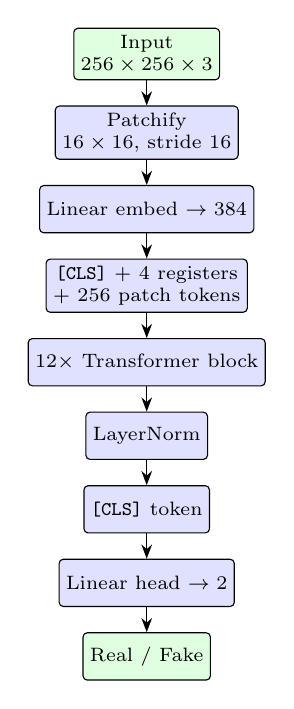
\begin{tikzpicture}[node distance=3.2mm]
\node[tensor] (img) {Input\\$256\times256\times3$};
\node[vit, below=of img] (patch) {Patchify\\$16\times16$, stride $16$};
\node[vit, below=of patch] (proj) {Linear embed $\to 384$};
\node[vit, below=of proj] (toks) {\texttt{[CLS]} + 4 registers\\+ 256 patch tokens};
\node[vit, below=of toks] (blocks) {$12\times$ Transformer block};
\node[vit, below=of blocks] (ln) {LayerNorm};
\node[vit, below=of ln] (cls) {\texttt{[CLS]} token};
\node[vit, below=of cls] (head) {Linear head $\to 2$};
\node[tensor, below=of head] (out) {Real / Fake};
\foreach \from/\to in {img/patch, patch/proj, proj/toks, toks/blocks, blocks/ln, ln/cls, cls/head, head/out}
  \draw[arr] (\from) -- (\to);
\end{tikzpicture}
\caption{ViT pipeline}
\label{fig:vit_pipe}
\end{subfigure}\hfill
\begin{subfigure}[b]{0.46\textwidth}
\centering
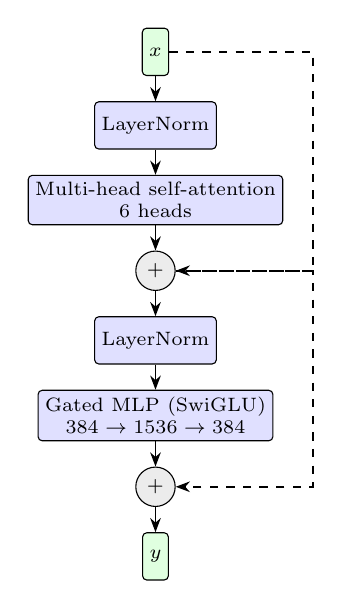
\begin{tikzpicture}[node distance=3.2mm]
\node[tensor] (x) {$x$};
\node[vit, below=of x] (ln1) {LayerNorm};
\node[vit, below=of ln1] (mhsa) {Multi-head self-attention\\$6$ heads};
\node[op, below=of mhsa] (add1) {$+$};
\node[vit, below=of add1] (ln2) {LayerNorm};
\node[vit, below=of ln2] (mlp) {Gated MLP (SwiGLU)\\$384\to1536\to384$};
\node[op, below=of mlp] (add2) {$+$};
\node[tensor, below=of add2] (y) {$y$};
\coordinate (lane) at ([xshift=2.0cm]x.center);
\draw[arr] (x) -- (ln1);
\draw[arr] (ln1) -- (mhsa);
\draw[arr] (mhsa) -- (add1);
\draw[arr] (add1) -- (ln2);
\draw[arr] (ln2) -- (mlp);
\draw[arr] (mlp) -- (add2);
\draw[arr] (add2) -- (y);
\draw[res] (x.east) -- (lane |- x.east) |- (add1.east);
\draw[res] (add1.east) -- (lane |- add1.east) |- (add2.east);
\end{tikzpicture}
\caption{Transformer block (gated variant)}
\label{fig:vit_block}
\end{subfigure}
\caption{\textbf{DINOv3 ViT-S/16 (Plus).} (a) Full pipeline: the image is split into $16\times16$
patches, embedded to $384$ dimensions, prepended with a \texttt{[CLS]} token and $4$ register
tokens, and passed through $12$ transformer blocks; the final \texttt{[CLS]} embedding is
classified by a linear head. (b) One transformer block, with a gated (SwiGLU) MLP and residual
connections around both sub-layers.}
\label{fig:vit_arch}
\end{figure}


\begin{figure}[H]
\centering
\begin{subfigure}[b]{0.46\textwidth}
\centering
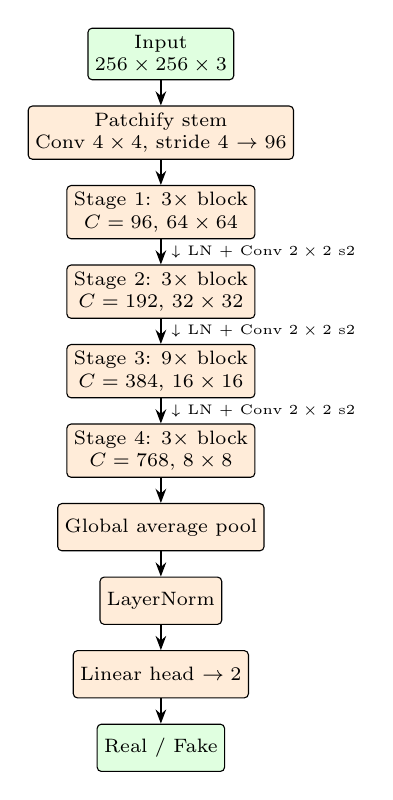
\begin{tikzpicture}[node distance=3.2mm]
\node[tensor] (img) {Input\\$256\times256\times3$};
\node[cnn, below=of img] (stem) {Patchify stem\\Conv $4\times4$, stride $4$ $\to 96$};
\node[cnn, below=of stem] (s1) {Stage 1: $3\times$ block\\$C=96$, $64\times64$};
\node[cnn, below=of s1] (s2) {Stage 2: $3\times$ block\\$C=192$, $32\times32$};
\node[cnn, below=of s2] (s3) {Stage 3: $9\times$ block\\$C=384$, $16\times16$};
\node[cnn, below=of s3] (s4) {Stage 4: $3\times$ block\\$C=768$, $8\times8$};
\node[cnn, below=of s4] (gap) {Global average pool};
\node[cnn, below=of gap] (ln) {LayerNorm};
\node[cnn, below=of ln] (head) {Linear head $\to 2$};
\node[tensor, below=of head] (out) {Real / Fake};
\draw[arr] (img) -- (stem);
\draw[arr] (stem) -- (s1);
\draw[arr] (s1) -- node[right, font=\tiny]{$\downarrow$ LN + Conv $2\times2$ s2} (s2);
\draw[arr] (s2) -- node[right, font=\tiny]{$\downarrow$ LN + Conv $2\times2$ s2} (s3);
\draw[arr] (s3) -- node[right, font=\tiny]{$\downarrow$ LN + Conv $2\times2$ s2} (s4);
\draw[arr] (s4) -- (gap);
\draw[arr] (gap) -- (ln);
\draw[arr] (ln) -- (head);
\draw[arr] (head) -- (out);
\end{tikzpicture}
\caption{ConvNeXt pipeline}
\label{fig:cnn_pipe}
\end{subfigure}\hfill
\begin{subfigure}[b]{0.46\textwidth}
\centering
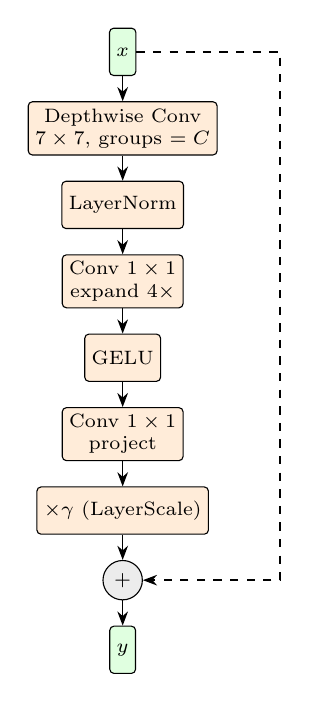
\begin{tikzpicture}[node distance=3.2mm]
\node[tensor] (x) {$x$};
\node[cnn, below=of x] (dw) {Depthwise Conv\\$7\times7$, groups $=C$};
\node[cnn, below=of dw] (ln) {LayerNorm};
\node[cnn, below=of ln] (pw1) {Conv $1\times1$\\expand $4\times$};
\node[cnn, below=of pw1] (gelu) {GELU};
\node[cnn, below=of gelu] (pw2) {Conv $1\times1$\\project};
\node[cnn, below=of pw2] (ls) {$\times\gamma$ (LayerScale)};
\node[op, below=of ls] (add) {$+$};
\node[tensor, below=of add] (y) {$y$};
\coordinate (lane) at ([xshift=2.0cm]x.center);
\draw[arr] (x) -- (dw);
\draw[arr] (dw) -- (ln);
\draw[arr] (ln) -- (pw1);
\draw[arr] (pw1) -- (gelu);
\draw[arr] (gelu) -- (pw2);
\draw[arr] (pw2) -- (ls);
\draw[arr] (ls) -- (add);
\draw[arr] (add) -- (y);
\draw[res] (x.east) -- (lane |- x.east) |- (add.east);
\end{tikzpicture}
\caption{ConvNeXt block}
\label{fig:cnn_block}
\end{subfigure}
\caption{\textbf{DINOv3 ConvNeXt-Tiny.} (a) Full pipeline: a patchify stem followed by four
stages with depths $[3,3,9,3]$ and widths $[96,192,384,768]$, separated by $2\times2$ stride-$2$
downsampling layers, ending in global average pooling and a linear head. (b) One ConvNeXt block:
a $7\times7$ depthwise convolution, layer normalization, an inverted bottleneck ($1\times1$,
expand $4\times$, GELU, $1\times1$), LayerScale, and a residual connection.}
\label{fig:cnn_arch}
\end{figure}


\subsection{Evaluation Protocol}
To isolate the effect of the backbone architecture, we freeze both backbones and train a
\emph{linear probe}---a logistic regression classifier with $L_2$ regularization and balanced
class weights---on top of the extracted features. Inputs are resized to $256\times256$ and
normalized with ImageNet statistics. The probe is trained on the training split and evaluated on
the identity-disjoint test split. Reported metrics are accuracy, precision, recall, F1, and
ROC-AUC, with \emph{fake} treated as the positive class.

For the fine-tuning experiment, we attach a single linear classification head to the frozen
backbone and train the full model (backbone + head) end-to-end with a low learning rate for the
backbone ($10^{-5}$) and a higher learning rate for the head ($10^{-3}$), using AdamW with
weight decay and cosine annealing. Full details are reported with the results.

\subsection{Datasets}
\textbf{DeepFakeFace} is used for the primary benchmark. It contains roughly $120$k images across
real (wiki) faces and three families of fakes (insight, inpainting, and text-to-image). We use an
identity-disjoint split (train / validation / test partitioned by person) to prevent the model
from exploiting identity-level leakage. For the controlled comparison we use the balanced
``insight'' split ($43{,}294$ train / $11{,}920$ test samples).

\textbf{DeepfakeTIMIT} is used as an auxiliary, out-of-distribution evaluation. All $640$ videos
are faceswapped (i.e., fake), so we report the \emph{detection rate}---the fraction of extracted
frames correctly flagged as fake---rather than a full accuracy score, since no real class is
present.

\textbf{FaceForensics++ benchmark} ($1000$ unlabeled compressed images) is used qualitatively to
probe cross-domain generalization; because labels are withheld, no quantitative score is reported.

\section{Experiments and Results}

\subsection{Experiment 1: Matched-Parameter Linear-Probe Comparison on DeepFakeFace}
We first compare the backbones at their natural scales by training a linear probe on frozen
features. Table~\ref{tab:deepfakeface} reports performance on the identity-disjoint DeepFakeFace
test split, and Figure~\ref{fig:linprobe} visualizes the same metrics for the matched-parameter
pair.

\begin{table}[H]
\centering
\caption{Linear-probe performance on DeepFakeFace (identity-disjoint test split). Both models
are frozen \textsc{DINOv3} backbones; the probe is logistic regression.}
\label{tab:deepfakeface}
\begin{tabular}{lcccccc}
\toprule
\textbf{Model} & \textbf{Params} & \textbf{Acc.} & \textbf{Prec.} & \textbf{Rec.} & \textbf{F1} & \textbf{AUC} \\
\midrule
ViT-S/16 (std.\ MLP)      & $21.6$M & $67.4\%$ & $67.7\%$ & $66.5\%$ & $67.1\%$ & $73.8\%$ \\
ViT-S/16 (Plus, gated)    & $28.7$M & $73.8\%$ & $73.2\%$ & $75.0\%$ & $74.1\%$ & $81.6\%$ \\
ConvNeXt-Tiny             & $27.8$M & $74.5\%$ & $74.0\%$ & $75.5\%$ & $74.7\%$ & $82.0\%$ \\
\bottomrule
\end{tabular}
\end{table}

\begin{figure}[H]
\centering

\includegraphics[width=0.78\textwidth]{linprobe_comparison.png}
\caption{Linear-probe metrics for the matched-parameter pair (ViT-S/16 Plus, $28.7$M, vs.\
ConvNeXt-Tiny, $27.8$M) on the DeepFakeFace identity-disjoint test split.}
\label{fig:linprobe}
\end{figure}

Two observations follow directly. First, the gated MLP confers a substantial improvement to the
ViT: moving from the standard MLP ($21.6$M) to the gated variant ($28.7$M) raises accuracy by
$+6.4$ points ($67.4\% \to 73.8\%$). Second, at a \emph{matched} parameter count ($28.7$M vs.\
$27.8$M), the ViT and the ConvNeXt are statistically indistinguishable, differing by only $0.7$
points of accuracy and $0.7$ points of F1. This is the central result of the study: once scale,
pretraining signal, and teacher are controlled, the architectural choice between ViT and CNN has
little effect on a diverse, modern manipulation benchmark.

\subsection{Experiment 2: End-to-End Fine-Tuning of the ViT}\label{sec:finetune}
The linear probe measures the quality of the \emph{frozen} features but leaves the full capacity
of the backbone untapped. We therefore fine-tune the standard ViT-S/16 ($21.6$M) end-to-end for
five epochs on the same ``insight'' split, keeping the backbone learning rate low to preserve the
pretrained representations. Figure~\ref{fig:finetune_loss} shows the training dynamics: the train
loss falls from $0.346$ to $0.046$ while validation accuracy climbs from $88.5\%$ to $96.5\%$,
indicating fast, stable convergence without overfitting.

\begin{figure}[H]
\centering

\includegraphics[width=0.72\textwidth]{finetune_loss.png}
\caption{Fine-tuning dynamics of DINOv3 ViT-S/16 over five epochs. Left axis (blue): train loss;
right axis (red/gray): validation accuracy and F1.}
\label{fig:finetune_loss}
\end{figure}

Table~\ref{tab:finetune} contrasts fine-tuning against the linear probe on the \emph{same}
backbone. End-to-end fine-tuning raises accuracy by $+28.9$ points ($67.4\% \to 96.3\%$) and
ROC-AUC by $+25.6$ points ($73.8\% \to 99.4\%$), confirming that the frozen linear probe
substantially understates what the pretrained backbone can achieve once its weights are adapted to
the target distribution.

\begin{table}[H]
\centering
\caption{Fine-tuning vs.\ linear probe on the same ViT-S/16 backbone (DeepFakeFace ``insight''
split, identity-disjoint test).}
\label{tab:finetune}
\begin{tabular}{lcccccc}
\toprule
\textbf{Setting} & \textbf{Acc.} & \textbf{Prec.} & \textbf{Rec.} & \textbf{F1} & \textbf{AUC} \\
\midrule
Linear probe (frozen)   & $67.4\%$ & $67.7\%$ & $66.5\%$ & $67.1\%$ & $73.8\%$ \\
Fine-tuned (5 epochs)   & $96.3\%$ & $96.3\%$ & $96.3\%$ & $96.3\%$ & $99.4\%$ \\
\bottomrule
\end{tabular}
\end{table}

\begin{figure}[H]
\centering

\includegraphics[width=0.42\textwidth]{finetune_cm.png}
\caption{Confusion matrix of the fine-tuned ViT on the $11{,}920$-sample test set. Rows are true
labels, columns are predictions; \emph{fake} is the positive class.}
\label{fig:finetune_cm}
\end{figure}

The confusion matrix (Figure~\ref{fig:finetune_cm}) is nearly diagonal: only $218$ real images are
misclassified as fake and $223$ fake images as real, out of $11{,}920$ samples. The model is
balanced across classes (precision $96.3\%$ vs.\ recall $96.3\%$), with no sign of the class
imbalance that can degrade a linear probe. We note that, because the fine-tuned standard ViT
($21.6$M) already exceeds the linear-probe Plus variant ($28.7$M) by a wide margin, the natural
next step is to fine-tune the ConvNeXt and the gated ViT under identical settings---the paired
fine-tuning comparison is left as future work (Section~\ref{sec:future}).

\subsection{Experiment 3: Out-of-Distribution Detection on DeepfakeTIMIT}
To stress-test the inductive biases further, we evaluate both backbones on DeepfakeTIMIT, an older
faceswap-GAN dataset whose manipulations exhibit coarse, local blending artifacts. Because every
video is fake, we report the detection rate in Table~\ref{tab:df_timit} and
Figure~\ref{fig:timit}, further broken down by quality level (HQ: $128\times128$ swaps; LQ:
$64\times64$ swaps).

\begin{table}[H]
\centering
\caption{Detection rate on DeepfakeTIMIT (all $640$ videos are faceswapped / fake). A higher
rate means more frames are correctly flagged as fake.}
\label{tab:df_timit}
\begin{tabular}{lcccc}
\toprule
\textbf{Model} & \textbf{Overall} & \textbf{HQ} & \textbf{LQ} & \textbf{Mean $p(\text{fake})$} \\
\midrule
ViT-S/16 (Plus)   & $75.8\%$ & $65.6\%$ & $85.9\%$ & $0.653$ \\
ConvNeXt-Tiny     & $98.9\%$ & $99.1\%$ & $98.8\%$ & $0.895$ \\
\bottomrule
\end{tabular}
\end{table}

\begin{figure}[H]
\centering

\includegraphics[width=0.68\textwidth]{timit_detection.png}
\caption{DeepfakeTIMIT detection rate by quality level. The ConvNeXt is near-perfect and robust
across quality, whereas the ViT degrades sharply on high-quality swaps.}
\label{fig:timit}
\end{figure}

Here the architectures diverge sharply: the ConvNeXt detects $98.9\%$ of the fake frames, whereas
the ViT detects only $75.8\%$. Moreover, the ViT's performance is quality-dependent---it performs
much worse on high-quality swaps ($65.6\%$) than on low-quality ones ($85.9\%$)---whereas the
ConvNeXt is robust across both quality levels ($99.1\%$ / $98.8\%$). Figure~\ref{fig:timit_hist}
offers a complementary view: the ConvNeXt's per-frame confidence is sharply concentrated near
$p(\text{fake})=1$, while the ViT's confidence is spread across the full $[0,1]$ range. This
supports the hypothesis that the convolutional backbone, with its local receptive fields, is
better equipped to capture the low-level blending seams and color inconsistencies that
characterize early-generation faceswaps, whereas the transformer's global attention is
comparatively insensitive to these subtle, spatially localized cues.

\begin{figure}[H]
\centering

\includegraphics[width=0.82\textwidth]{timit_prob_hist.png}
\caption{Distribution of predicted $p(\text{fake})$ over the $640$ DeepfakeTIMIT frames. The
dashed line marks the $0.5$ decision boundary. The ConvNeXt is confidently correct; the ViT is
uncertain on a large fraction of frames.}
\label{fig:timit_hist}
\end{figure}

\subsection{Experiment 4: Attention Visualization}
To probe \emph{where} the ViT looks when classifying a face, we extract the \texttt{[CLS]}-to-patch
attention from selected layers (5, 8, and 11), average across the $6$ heads, and overlay the
resulting heatmap on the input image (Figure~\ref{fig:attention}). Two patterns emerge. First,
attention is spatially diffuse in early layers and progressively concentrates on the face interior
(eyes, nose, mouth) in deeper layers, consistent with the transition from local texture to global
semantic grouping that ViTs are known to undergo. Second, the attended regions differ qualitatively
between real and fake inputs, suggesting that the transformer keys in on identity- and
structure-related cues rather than the localized blending seams that a CNN exploits. This is the
spatial counterpart of the quantitative result in Experiment 3: the two architectures look at
different evidence, and they therefore fail on different distributions.

\begin{figure}[H]
\centering

\includegraphics[width=\textwidth]{attention_grid.png}
\caption{DINOv3 ViT attention maps (CLS token, averaged over heads) for a matched real/fake pair
at layers 5, 8, and 11. Deeper layers concentrate attention on facial structure; the attended
regions differ between real and fake inputs.}
\label{fig:attention}
\end{figure}

\subsection{Experiment 5: Cross-Domain Probe on FaceForensics++}
Finally, we probe generalization to the FaceForensics++ benchmark ($1000$ unlabeled, heavily
compressed images). Without ground-truth labels no accuracy can be computed; however, the two
models agree on only $58\%$ of images and both produce near-random confidence distributions
(mean predicted fake probability $\approx0.53$), indicating that features learned on DeepFakeFace
do not transfer well to this distribution. This is consistent with the known difficulty of
cross-dataset generalization in deepfake detection and highlights the importance of in-domain
training for benchmark-grade performance.

\section{Discussion}

\subsection{Why Convolution Wins on Old, Coarse Artifacts}
The divergent behavior on DeepfakeTIMIT is instructive. Faceswap-GAN (2018) produces artifacts
that are \emph{local} and \emph{low-level}: visible seams at the face boundary, slight color
mismatches between the swapped face and the surrounding skin, and blurring around the mouth and
eyes. A depthwise $7\times7$ convolution is precisely tuned to detect such local texture
statistics, and the hierarchical nature of ConvNeXt (shallow stages for fine detail, deep stages
for semantics) mirrors the multi-scale structure of these artifacts. In contrast, a ViT's
self-attention aggregates information globally from the outset, which can dilute spatially
localized but diagnostically important cues---as corroborated by the diffuse, semantics-driven
attention maps in Figure~\ref{fig:attention}.

\subsection{Why the Gap Disappears on Modern, Diverse Data}
On DeepFakeFace---which spans three modern generator families with more subtle, diverse, and
semantic manipulations---the architectures converge to a near-tie. We attribute this to two
factors. First, modern manipulations leave fewer consistent low-level artifacts, shifting the
discriminative signal toward higher-level, identity- and structure-related cues that attention
models capture well. Second, the matched parameter count and shared DINOv3 pretraining remove the
confounding scale advantages that would otherwise favor one architecture, leaving a fair test in
which neither inductive bias dominates.

\subsection{The Role of Fine-Tuning}
The fine-tuning experiment reframes the linear-probe comparison. Under a frozen linear probe, the
two backbones sit near $74\%$ F1; once the ViT is fine-tuned, it reaches $96.3\%$ accuracy with a
near-diagonal confusion matrix. This implies that the ``architecture matters little'' conclusion
is a property of the \emph{linear-probe} regime: the pretrained features of both backbones are
comparably discriminative, but each still holds substantial task-specific capacity that only
adaptation releases. A complete architecture comparison therefore requires matched fine-tuning of
both backbones, which we leave to future work.

\subsection{Limitations}
Our study has several limitations. (i) The linear-probe results measure the quality of the
pretrained features but not the full capacity of fine-tuned models; only the ViT is fine-tuned
here. (ii) The evaluation is image-level; temporal (video-level) artifacts---flicker, unnatural
blinking, frame-to-frame inconsistency---are ignored, and these are often the strongest cues in
real-world deepfakes. (iii) The DeepfakeTIMIT evaluation is one-sided (no real class), so it
reports detection rate rather than a balanced accuracy. (iv) Cross-domain results are qualitative
only. Each of these is a natural target for future work.

\section{Conclusion and Future Work}
We implemented a Vision Transformer and a ConvNeXt backbone, both initialized from \textsc{DINOv3}
self-supervised weights, and compared them for deepfake detection under a matched parameter budget
of approximately $28$M parameters. Our key findings are: (1) at matched scale, ViT and CNN perform
nearly identically on a diverse modern manipulation benchmark ($74.1\%$ vs.\ $74.5\%$ F1);
(2) the gated MLP improves the ViT by $+6.4$ accuracy points; (3) the convolutional backbone
substantially outperforms the transformer on an older faceswap-GAN dataset ($98.9\%$ vs.\ $75.8\%$
detection rate), supporting the view that convolution is better suited to local, low-level
artifacts while attention excels at semantic reasoning; and (4) end-to-end fine-tuning of the ViT
lifts accuracy from $67.4\%$ to $96.3\%$, showing that the architecture gap is largely a property
of the linear-probe regime.

\subsection{Future Work}\label{sec:future}
Future work will extend this comparison in several directions. First, we will complete the
\emph{matched fine-tuning} of both backbones (the paired fine-tuning script already exists) to
test whether the ConvNeXt retains its edge on older artifacts once adapted. Second, we will move
from image-level to \emph{video-level} detection by aggregating predictions across multiple frames
per video (late fusion) or by introducing temporal models (3D convolutions or temporal
transformers), which can exploit motion cues that single frames cannot reveal. Third, we will
evaluate cross-dataset generalization on FaceForensics++ and Celeb-DF under fine-tuning, which
remains the most practically meaningful test of a deepfake detector.

\bibliographystyle{plain}
\begin{thebibliography}{9}

\bibitem{dosovitskiy2021vit}
A. Dosovitskiy, L. Beyer, A. Kolesnikov, D. Weissenborn, X. Zhai, T. Unterthiner,
M. Dehghani, M. Minderer, G. Heigold, S. Gelly, J. Uszkoreit, and N. Houlsby.
An image is worth $16\times16$ words: Transformers for image recognition at scale.
\emph{International Conference on Learning Representations (ICLR)}, 2021.

\bibitem{liu2022convnext}
Z. Liu, H. Mao, C.-Y. Wu, C. Feichtenhofer, T. Darrell, and S. Xie.
A ConvNet for the 2020s.
\emph{IEEE/CVF Conference on Computer Vision and Pattern Recognition (CVPR)}, 2022.

\bibitem{dinov3}
Meta AI. DINOv3: Scaling self-supervised learning for vision foundation models.
arXiv:2508.10104, 2025.

\bibitem{rossler2019faceforensics}
A. R\"ossler, D. Cozzolino, L. Verdoliva, C. Riess, J. Thies, and M. Nie{\ss}ner.
FaceForensics++: Learning to detect manipulated facial images.
\emph{IEEE/CVF International Conference on Computer Vision (ICCV)}, 2019.

\bibitem{korshunov2018deepfakes}
P. Korshunov and S. Marcel.
DeepFakes: a new threat to face recognition? Assessment and detection.
arXiv:1812.08685, 2018.

\bibitem{chollet2017xception}
F. Chollet.
Xception: Deep learning with depthwise separable convolutions.
\emph{IEEE/CVF Conference on Computer Vision and Pattern Recognition (CVPR)}, 2017.

\end{thebibliography}

\end{document}
